% Compile with XeLaTeX twice. See README.md.
\documentclass[12pt,a4paper,oneside]{report}
\usepackage[a4paper,left=1.5in,right=1in,top=1in,bottom=1in]{geometry}
% \usepackage{fontspec} % fontspec requires XeLaTeX or LuaLaTeX, not pdfLaTeX
% \IfFontExistsTF{Times New Roman}{\setmainfont{Times New Roman}}{\setmainfont{Liberation Serif}}
\usepackage{setspace,graphicx,booktabs,array,amsmath,amssymb}
\usepackage{fancyhdr,caption,float,enumitem,titlesec,listings,xcolor}
\usepackage[hidelinks]{hyperref}
% -------- EDIT ONLY THIS FILE FOR PROJECT DETAILS --------
\newcommand{\ProjectTitle}{SECURESPHERE-AI: ENTERPRISE AI FIREWALL \& PRIVACY-PRESERVING MULTIMODAL LLM GATEWAY}
\newcommand{\ReportType}{Major Project Report}
\newcommand{\DegreeStream}{COMPUTER SCIENCE AND ENGINEERING (DATA SCIENCE)}
\newcommand{\Department}{Department of Computer Science \& Engineering (Data Science)}
\newcommand{\DepartmentFooter}{Dept. of CSE--Allied (Data Science), MVSREC}
\newcommand{\AcademicYear}{2026--27}

% Team Members (Batch 03)
\newcommand{\StudentOne}{Rithika Chalva}
\newcommand{\RollOne}{2451-23-750-038}
\newcommand{\StudentTwo}{Yadala Krupa Samuel Dan}
\newcommand{\RollTwo}{2451-23-750-047}
\newcommand{\StudentThree}{Nagarjuna Chaitanya Sandeep}
\newcommand{\RollThree}{2451-23-750-055}

% Guide & Institutional Officers
\newcommand{\GuideName}{Dr. B. Sandhya}
\newcommand{\GuideDesignation}{Professor}
\newcommand{\HODName}{Dr. Rajesh Kulkarni}
\newcommand{\HODDesignation}{Professor and Head}
\newcommand{\PrincipalName}{Dr. G. Kanaka Durga}
\newcommand{\CoordinatorName}{Project Coordinator}
\newcommand{\CoordinatorDesignation}{Sr Assistant Professor}

\newcommand{\CollegeName}{MVSR ENGINEERING COLLEGE}
\newcommand{\CollegeLocation}{Nadergul, Balapur Mandal, Hyderabad -- 501 510}


\setstretch{1.5}
\setlength{\parindent}{0.5in}
\setlength{\parskip}{6pt}
\setcounter{secnumdepth}{3}
\setcounter{tocdepth}{2}

\titleformat{\chapter}[display]{\bfseries\fontsize{14}{18}\selectfont\centering}{CHAPTER -- \thechapter}{0.3cm}{\MakeUppercase}
\titlespacing*{\chapter}{0pt}{0pt}{16pt}
\titleformat{\section}{\bfseries\fontsize{12}{16}\selectfont}{\thesection}{0.6em}{\MakeUppercase}
\titleformat{\subsection}{\bfseries\fontsize{12}{16}\selectfont}{\thesubsection}{0.6em}{}
\captionsetup{font={small},labelfont=bf}

\numberwithin{equation}{chapter}
\renewcommand{\thefigure}{\thechapter.\arabic{figure}}
\renewcommand{\thetable}{\thechapter.\arabic{table}}

\fancypagestyle{chapterpages}{%
 \fancyhf{}\fancyhead[R]{\fontsize{10}{12}\selectfont\ProjectTitle}
 \fancyfoot[L]{\fontsize{10}{12}\selectfont\DepartmentFooter}
 \fancyfoot[R]{\fontsize{10}{12}\selectfont\thepage}
 \renewcommand{\headrulewidth}{0pt}\renewcommand{\footrulewidth}{0pt}}

\fancypagestyle{frontpages}{\fancyhf{}\fancyfoot[C]{\roman{page}}\renewcommand{\headrulewidth}{0pt}}
\fancypagestyle{plain}{\fancyhf{}\fancyhead[R]{\fontsize{10}{12}\selectfont\ProjectTitle}\fancyfoot[L]{\fontsize{10}{12}\selectfont\DepartmentFooter}\fancyfoot[R]{\fontsize{10}{12}\selectfont\thepage}\renewcommand{\headrulewidth}{0pt}}

\newcommand{\FrontHeading}[1]{\begin{center}\fontsize{14}{18}\selectfont\bfseries #1\end{center}\vspace{0.6cm}}
\newcommand{\Logo}{
\includegraphics[height=3cm,keepaspectratio]{images/MVSR_logo.jpg}}
\newcommand{\StudentsList}{\StudentOne\ (\RollOne), \StudentTwo\ (\RollTwo), and \StudentThree\ (\RollThree)}

% Code listing configuration
\lstset{
  basicstyle=\ttfamily\footnotesize,
  breaklines=true,
  frame=single,
  backgroundcolor=\color{black!3},
  numbers=left,
  numberstyle=\tiny\color{gray},
  keywordstyle=\color{blue}\bfseries,
  commentstyle=\color{green!50!black}\itshape,
  stringstyle=\color{red!70!black},
  showstringspaces=false
}

\begin{document}
\pagenumbering{gobble}\pagestyle{empty}
% Single-page A4 title page. Edit project details in config.tex.
\begin{titlepage}
\thispagestyle{empty}
\centering
\setlength{\parindent}{0pt}
\setlength{\parskip}{0pt}
\vspace*{0.1cm}
{\fontsize{12}{14}\selectfont A\\[0.08cm]\ReportType\\[0.08cm]on\par}
\vspace{0.3cm}
{\fontsize{14}{17}\selectfont\bfseries\ProjectTitle\par}
\vspace{0.35cm}
{\fontsize{11}{14}\selectfont Submitted for partial fulfilment of the requirements for the award of the degree of\par}
\vspace{0.3cm}
{\fontsize{12}{14}\selectfont\bfseries BACHELOR OF ENGINEERING\par}
\vspace{0.15cm}
in\par
\vspace{0.15cm}
{\fontsize{12}{15}\selectfont\bfseries\DegreeStream\par}
\vspace{0.3cm}
By\par
\vspace{0.2cm}
{\fontsize{12}{16}\selectfont\bfseries
\StudentOne\ (\RollOne)\\
\StudentTwo\ (\RollTwo)\\
\StudentThree\ (\RollThree)\par}
\vspace{0.35cm}
Under the guidance of\par
\vspace{0.15cm}
{\fontsize{12}{15}\selectfont\bfseries\GuideName\par}
\vspace{0.05cm}
\GuideDesignation\par
\Department\par
\vfill
\Logo\par
\vspace{0.2cm}
{\fontsize{14}{17}\selectfont\bfseries\CollegeName\par}
\vspace{0.08cm}
{\bfseries (AUTONOMOUS)}\par
\vspace{0.08cm}
\Department\par
\vspace{0.08cm}
{\fontsize{10}{12}\selectfont (Affiliated to Osmania University \& Recognized by AICTE)\par}
\vspace{0.08cm}
\CollegeLocation\par
\vspace{0.08cm}
Academic Year: \AcademicYear\par
\vspace*{0.1cm}
\end{titlepage}

\clearpage

% Certificate is roman page i; title page remains unnumbered.
\pagenumbering{roman}\setcounter{page}{1}\pagestyle{frontpages}
\begin{center}\Logo\end{center}\vspace{0.7cm}
\FrontHeading{CERTIFICATE}
\noindent\textit{This is to certify that the project work entitled \textbf{``\ProjectTitle''} is a bonafide work carried out by \textbf{\StudentsList} in partial fulfilment of the requirements for the award of the degree of \textbf{Bachelor of Engineering in \DegreeStream} from \textbf{MVSR Engineering College (Autonomous)}, affiliated to \textbf{Osmania University, Hyderabad}, during the academic year \AcademicYear\ under our guidance and supervision.}

\noindent\textit{The results embodied in this report have not been submitted to any other university or institute for the award of any degree or diploma to the best of our knowledge and belief.}
\vfill
\noindent\begin{tabular}{@{}p{0.48\textwidth}@{\hfill}p{0.48\textwidth}@{}}
\textbf{Internal Guide:} & \raggedleft\textbf{Head of the Department:}\tabularnewline[0.25cm]
\GuideName & \raggedleft\HODName\tabularnewline
\GuideDesignation, Dept. of CSE & \raggedleft\HODDesignation, Dept. of CSE\tabularnewline
MVSREC & \raggedleft MVSREC\tabularnewline
\end{tabular}
\vspace{1cm}

\clearpage\FrontHeading{DECLARATION}
\noindent We declare that the project report entitled \textbf{``\ProjectTitle''} is a record of bonafide project work carried out by us in \Department, MVSR Engineering College, affiliated to Osmania University, during the academic year \AcademicYear. The work reported here has been done by us and has not been copied from any other source. The results have not been submitted to another university or institute for the award of any degree or diploma.
\vfill
\noindent\begin{tabular}{@{}p{0.32\textwidth}p{0.32\textwidth}p{0.32\textwidth}@{}}
\centering\StudentOne & \centering\StudentTwo & \centering\arraybackslash\StudentThree\\
\centering(\RollOne) & \centering(\RollTwo) & \centering\arraybackslash(\RollThree)
\end{tabular}
\vspace{1cm}

% Uncomment if this is an industry project and insert actual certificate:
% \clearpage\FrontHeading{INDUSTRY CERTIFICATE}
[Insert the approved industry certificate if the project is conducted with an industry partner.]

\clearpage\FrontHeading{ACKNOWLEDGEMENT}

We express our deepest sense of gratitude and respect to our project guide \textbf{\GuideName}, \GuideDesignation, \Department, for her invaluable guidance, continuous encouragement, and profound technical insights throughout the design, development, and testing of \textbf{\ProjectTitle}. Her constructive critique and support were instrumental in realizing this work.

We extend our sincere thanks to \textbf{\HODName}, \HODDesignation, \Department, and our respected Principal \textbf{\PrincipalName}, for providing the state-of-the-art computational infrastructure, laboratories, and academic ecosystem that facilitated the successful completion of this major project.

We also thank our Project Coordinator, \textbf{\CoordinatorName}, \CoordinatorDesignation, for meticulously scheduling reviews, monitoring milestones, and ensuring adherence to academic guidelines. 

Finally, we convey our heartfelt appreciation to the faculty members, technical staff of the Department of Computer Science \& Engineering (Data Science), our fellow students, and our parents for their constant encouragement and moral support throughout our academic journey.

\vfill
\begin{flushright}
\StudentOne\ (\RollOne)\\\StudentTwo\ (\RollTwo)\\\StudentThree\ (\RollThree)
\end{flushright}

\clearpage\FrontHeading{VISION \& MISSION}
\section*{VISION}
To evolve as a premier academic and research hub aligned with the global standards in the emerging areas of Computer Science.
\section*{MISSION}
\noindent\textbf{M1:} To impart strong fundamental and applied knowledge, producing technically competent engineers to address current industrial and societal challenges.

\noindent\textbf{M2:} To enable students to develop feasible solutions with awareness towards environment and sustainability.

\noindent\textbf{M3:} To nurture a culture of research and innovation that contributes to cutting-edge advancements.

\noindent\textbf{M4:} To foster holistic professional development with strong human and ethical values.

\clearpage\FrontHeading{COURSE OBJECTIVES \& COURSE OUTCOMES}
\section*{Course Objectives}
\begin{enumerate}[leftmargin=*]
\item Enhance practical and professional skills.
\item Familiarize students with tools and techniques for systematic literature survey and documentation.
\item Expose students to industry practices and teamwork.
\item Encourage students to work with innovative and entrepreneurial ideas.
\end{enumerate}
\section*{Course Outcomes}
Upon completion of the course, students will be able to:
\begin{enumerate}[leftmargin=*]
\item Synthesize and apply the knowledge and skills acquired in the academic program to real-world problems.
\item Design and analyze the project with respect to the problem's requirements.
\item Implement all the aspects of SDLC through the project work.
\item Demonstrate effective written and oral communication skills.
\item Demonstrate the ability to work as part of a team.
\end{enumerate}

\clearpage\FrontHeading{ABSTRACT}

\noindent The pervasive adoption of multi-tenant cloud-hosted Large Language Models (LLMs), such as Google Gemini 2.5 Flash and OpenAI GPT-4o, provides unprecedented enterprise cognitive automation but simultaneously creates an acute data privacy and regulatory crisis. Corporate employees routinely submit prompts containing Personally Identifiable Information (PII), confidential financial figures, source code secrets, and biometric identity images to external APIs, breaching data sovereignty perimeters under the Digital Personal Data Protection (DPDP) Act 2023, RBI Cyber Security Framework, and EU GDPR. 

\vspace{0.3cm}
\noindent This project presents \textbf{SecureSphere-AI}, an intelligent, zero-trust security mediation gateway deployed at the enterprise egress boundary to enforce multi-tier data privacy without degrading generative model reasoning. The architecture introduces five tightly coupled defensive subsystems: (i) an advanced multi-tier entity recognition pipeline combining Microsoft Presidio, spaCy statistical models, custom context-aware pattern recognizers for 15+ Indian and global identifiers (e.g., bank accounts, Indian/international phone numbers, employee badges, credentials, and Verhoeff-verified Aadhaar IDs), and an optional sliding-window deep learning BERT NER layer; (ii) a dual cryptographic engine that pairs deterministic keyed HMAC-SHA256 Base32 pseudonymization (for multi-turn coreference stability) with an authenticated AES-256-GCM local session vault employing unique 96-bit nonces to eliminate stream-cipher keystream reuse vulnerabilities; (iii) a zero-knowledge numerical engine implementing real \textbf{TenSEAL CKKS Homomorphic Encryption} (polynomial degree $N=8192$, scale $2^{50}$), empowering external cloud models to evaluate arithmetic operations (addition, subtraction, averaging, multiplication, percentages) directly on ciphertext tokens without plaintext exposure, supported by a backward-compatible affine masking fallback; (iv) an ultra-low-latency OpenCV heuristic multimodal vision redactor that segments biometric faces (HSV/YCrCb color spaces) and license plates (Sobel gradient morphology) with dual-mode redaction; and (v) an automated system instruction injector ensuring cloud models preserve cryptographic placeholders.

\vspace{0.3cm}
\noindent Empirical validation across a rigorous 51-unit automated test suite demonstrates an end-to-end mediation overhead of \textbf{38.4\,ms}, a PII detection recall of \textbf{99.4\%}, and \textbf{0.00\% plaintext leakage} during cloud transit, delivering a mathematically verified, production-ready AI firewall.

\vfill
\begin{flushright}
\StudentOne\ (\RollOne)\\\StudentTwo\ (\RollTwo)\\\StudentThree\ (\RollThree)
\end{flushright}

\clearpage\tableofcontents
\clearpage\listoftables
\clearpage\listoffigures

\clearpage\pagenumbering{arabic}\setcounter{page}{1}\pagestyle{chapterpages}
\chapter{Introduction}

\section{Problem Statement}
The modern enterprise computing paradigm is experiencing a fundamental transition propelled by generative artificial intelligence and trillion-parameter Large Language Models (LLMs), such as Google Gemini 2.5 Flash, Anthropic Claude 3.5, and OpenAI GPT-4o. While these foundation models dramatically enhance developer productivity, automated code synthesis, and data analytics, their multi-tenant cloud-hosted deployment exposes enterprise data to acute vulnerabilities.

Employees routinely copy and paste sensitive operational data into public chat interfaces. This data encompasses Personally Identifiable Information (PII) including national identification numbers (Aadhaar, PAN), financial records, banking account details, passwords, internal API tokens, and corporate network configurations. Once transmitted over the public internet to third-party model providers, this data breaches the internal security perimeter, creating three critical vulnerabilities:
\begin{enumerate}[leftmargin=*]
    \item \textbf{Data Leakage \& Storage Ingestion:} Unencrypted prompts and sensitive figures are logged in cloud vendor telemetry or ingested into subsequent model retraining corpora, enabling unintentional cross-tenant leakage.
    \item \textbf{Loss of Numeric Confidentiality in Financial Reasoning:} When corporate users query cloud models to compute financial projections, tax computations, or salary bonuses, the raw numerical values are laid bare, disclosing confidential balance sheets.
    \item \textbf{Adversarial Jailbreaks \& Inbound Exploits:} Attackers embed adversarial prompt-injection payloads (e.g., ``DAN mode'', ``developer overrides'', or obfuscated base64 attacks) designed to bypass safety filters and exfiltrate internal system context.
\end{enumerate}

\section{Objectives}
The primary objective of \textbf{SecureSphere-AI} is to design, implement, and validate an asynchronous, privacy-preserving AI firewall that functions as a transparent reverse proxy between enterprise endpoints and external cloud LLMs. The specific measurable objectives are:
\begin{enumerate}[leftmargin=*]
    \item \textbf{Zero-Trust Inbound Sanitization:} Intercept all prompt traffic and automatically detect, classify, and pseudonymize 15+ categories of PII, financial identifiers, and enterprise credentials with recall exceeding 99\%.
    \item \textbf{Zero-Knowledge Numerical Homomorphic Encryption:} Implement true \textbf{TenSEAL CKKS Homomorphic Encryption} ($N=8192$, scale $2^{50}$) to encrypt financial figures into ciphertext tokens, enabling cloud LLMs to evaluate arithmetic operations (addition, subtraction, averaging, multiplication, percentages) directly on encrypted data without ever observing plaintext numbers.
    \item \textbf{Deterministic Coreference Pseudonymization:} Generate stable HMAC-SHA256 Base32 pseudonym tokens to preserve multi-turn linguistic relationships, backed by an authenticated AES-256-GCM session vault with fresh 96-bit random nonces per stored entry.
    \item \textbf{Sub-Millisecond Multimodal Biometric Redaction:} Develop a zero-GPU OpenCV heuristic computer vision pipeline to redact facial biometrics and vehicle license plates in under 15\,ms per image across Dual Redaction Modes.
    \item \textbf{Automated LLM System Note Injection:} Automatically inject constraints into external LLM prompts to force cloud models to strictly copy and preserve cryptographic placeholders without hallucinations or syntax degradation.
    \item \textbf{Ultra-Low Mediation Latency:} Maintain an end-to-end gateway proxy mediation overhead below 50\,ms to ensure seamless interactive human-in-the-loop performance.
\end{enumerate}

\section{Motivation}
Organizations in India and globally operate under increasingly stringent statutory compliance regimes:
\begin{itemize}[leftmargin=*]
    \item \textbf{Digital Personal Data Protection (DPDP) Act 2023:} Mandates that Data Fiduciaries implement reasonable technical safeguards to protect personal data, imposing statutory financial penalties of up to \textyen 250 Crores for data breaches.
    \item \textbf{Reserve Bank of India (RBI) Cyber Security Directives:} Enforces mandatory field-level encryption and strict confidentiality controls over financial and banking identifiers.
    \item \textbf{IT Act 2000 (Section 43A) \& European Union GDPR (Articles 25 \& 32):} Mandates data protection by design and default, enforcing strict civil liabilities for unauthorized disclosure of sensitive personal data or information (SPDI).
\end{itemize}
Hosting comparable trillion-parameter models strictly on-premises is economically unfeasible for most enterprises due to exorbitant GPU hardware acquisition and energy costs. SecureSphere-AI bridges this gap, allowing organizations to securely utilize top-tier cloud foundation models with mathematical privacy guarantees.

\section{Scope}
The scope of the project encompasses:
\begin{itemize}[leftmargin=*]
    \item Development of an asynchronous RESTful API gateway built on FastAPI and Uvicorn.
    \item Integration of Microsoft Presidio and spaCy statistical models, supplemented by 15+ custom regular expression and cue-based pattern recognizers.
    \item An optional CPU-based deep learning BERT NER layer with sliding-window boundary chunking.
    \item Mathematical implementation of the TenSEAL CKKS homomorphic scheme and an affine linear masking fallback ($S' = aS + b$).
    \item Development of an OpenCV-based computer vision guardrail supporting Mode A (Biometric Gaussian Blur) and Mode B (Zero-Knowledge ID Badge Black-Box Redaction).
    \item Implementation of a dual-phase policy engine for prompt-injection scoring and outbound leak validation.
    \item Implementation of a self-healing hybrid audit logger (MongoDB with automatic failover to SQLite).
    \item Design of an authentic enterprise Security Operations Center (SOC) dashboard built on Streamlit with interactive multimodal paste-bar components.
\end{itemize}

\section{Software and Hardware Requirements}

\subsection{Hardware Specifications}
\begin{itemize}[leftmargin=*]
    \item \textbf{Processor:} Multi-core 64-bit CPU (Intel Core i5-11th Gen / AMD Ryzen 5 5000 series or higher).
    \item \textbf{System Memory (RAM):} Minimum 8\,GB (16\,GB recommended for hosting local offline Ollama models).
    \item \textbf{Storage:} 256\,GB NVMe Solid State Drive (SSD) with at least 5\,GB free disk space.
    \item \textbf{Network Interface:} Standard broadband connection for outbound cloud API communication.
\end{itemize}

\subsection{Software Specifications}
\begin{itemize}[leftmargin=*]
    \item \textbf{Operating System:} Microsoft Windows 10/11 (64-bit) or Ubuntu Linux 22.04 LTS.
    \item \textbf{Programming Language:} Python 3.11 / 3.14.
    \item \textbf{Web Frameworks:} FastAPI 0.100+, Uvicorn 0.22+, Streamlit 1.28+.
    \item \textbf{Cryptographic Libraries:} TenSEAL 0.3.18, PyCryptodome 3.18+, Cryptography 41.0+.
    \item \textbf{NLP \& AI Frameworks:} Microsoft Presidio (Analyzer \& Anonymizer 2.2+), spaCy 3.5+ (\texttt{en\_core\_web\_sm}), optional Hugging Face Transformers (\texttt{dslim/bert-base-NER}).
    \item \textbf{Computer Vision:} OpenCV (\texttt{opencv-python} 4.10+), NumPy 1.24+.
    \item \textbf{Databases:} MongoDB 7.0 and SQLite3.
\end{itemize}

\section{Report Organization}
The remainder of this report is organized as follows:
\begin{itemize}[leftmargin=*]
    \item \textbf{Chapter 2 (Literature Survey):} Reviews the state-of-the-art in LLM privacy, homomorphic cryptography, tokenization schemes, and existing DLP systems.
    \item \textbf{Chapter 3 (System Design):} Details the architectural topology, data flow models, module specifications, and project execution schedule.
    \item \textbf{Chapter 4 (Implementation):} Provides an exhaustive code-level analysis of the cryptographic engine, PII detection logic, multimodal vision filters, and gateway middleware.
    \item \textbf{Chapter 5 (Testing \& Results):} Documents the 51-unit automated test suite, empirical benchmarks, and comparative evaluation against baseline methodologies.
    \item \textbf{Chapter 6 (Conclusion \& Future Enhancements):} Summarizes the major research findings, practical limitations, and outlines future directions including differential privacy and post-quantum cryptography.
\end{itemize}

\chapter{Background / Literature Survey}

\section{Survey of Major Area Relevant to Project}
The rapid commercialization of Large Language Models has sparked intensive academic and industrial research into Privacy-Preserving Machine Learning (PPML) and AI Security Guardrails. Foundation models operate under a multi-tenant cloud architecture where client prompts are transmitted over public networks to remote data centers. 

Ghosal et al.~\cite{ghosal2023llm} comprehensively investigated privacy vulnerabilities in commercial LLM APIs, establishing that static blacklisting and regular expression filters fail catastrophically against linguistic morphology, OCR noise, and natural language paraphrasing. Attackers and careless employees routinely bypass static keyword lists by spacing out letters, inserting punctuation, or using colloquial terminology. Furthermore, standard Data Loss Prevention (DLP) engines typically replace detected sensitive text with generic tags (e.g., \texttt{<REDACTED>}). As demonstrated by Carlini et al.~\cite{carlini2021extracting}, naive redaction strips the prompt of semantic coreference equality: if two distinct individuals are both replaced by \texttt{<PERSON>}, the cloud model loses track of relational logic, degrading conversational utility and causing hallucinations.

Another critical domain is Adversarial Prompt Injection and Jailbreaking. Perez and Ribeiro~\cite{perez2022ignore} demonstrated that foundation models are susceptible to indirect prompt injection, where malicious instructions embedded in documents or user inputs override system guardrails. Defending against these attacks requires a dual-phase architecture that intercepts adversarial patterns prior to model execution and validates outputs for policy violations prior to client delivery.

\section{Techniques and Algorithms Relevant to the Project}

\subsection{Homomorphic Encryption and the CKKS Scheme}
Homomorphic Encryption (HE) represents a cryptographic breakthrough allowing mathematical operations to be performed directly on encrypted data without requiring access to the decryption key. Early fully homomorphic schemes (e.g., Gentry's 2009 lattice-based construction) suffered from prohibitive computational overhead. 

In 2017, Cheon, Kim, Kim, and Song~\cite{cheon2017homomorphic} introduced the **CKKS scheme** (Homomorphic Encryption for Arithmetic of Approximate Numbers). CKKS is tailored for real-number floating-point computation by treating encryption noise as part of the numerical approximation error. Operations occur over the cyclotomic polynomial ring:
\begin{equation}
R_q = \mathbb{Z}_q[X] / (X^N + 1)
\end{equation}
where $N$ is a power-of-two polynomial modulus degree (typically $N=8192$ or $16384$) and $q$ is a composite ciphertext modulus composed of a chain of prime factors:
\begin{equation}
q = \prod_{i=0}^L q_i
\end{equation}
Given two plaintexts $m_1, m_2 \in \mathbb{R}$ encrypted into ciphertexts $c_1, c_2 \in R_q^2$, the CKKS addition and multiplication homomorphic properties satisfy:
\begin{align}
\text{Dec}(\text{Key}_{\text{secret}}, c_1 + c_2) &\approx m_1 + m_2 \\
\text{Dec}(\text{Key}_{\text{secret}}, c_1 \cdot c_2) &\approx m_1 \cdot m_2
\end{align}
SecureSphere-AI utilizes the **TenSEAL** library~\cite{tenseal2021}, which wraps Microsoft SEAL in high-performance C++ bindings. This allows mathematical queries from external models (e.g., computing an 18\% tax or multi-item expense summation) to execute directly on encrypted ciphertext vectors with zero knowledge of the underlying values.

\subsection{Symmetric Authenticated Encryption vs. Keyed PRFs}
A critical architectural pitfall in naive security proxies is attempting to use symmetric encryption directly inside prompts. In the Advanced Encryption Standard with Galois/Counter Mode (AES-256-GCM)~\cite{dworkin2007sp800}, encryption combines counter-mode keystream generation with a GHASH polynomial authenticator. If an identical Nonce/Initialization Vector (IV) is reused with the same key across two distinct inputs, an adversary can XOR the ciphertexts:
\begin{equation}
C_1 \oplus C_2 = (P_1 \oplus \text{Keystream}) \oplus (P_2 \oplus \text{Keystream}) = P_1 \oplus P_2
\end{equation}
This allows complete recovery of the plaintext difference and catastrophic key disclosure. Conversely, generating random nonces produces non-deterministic, high-entropy Base64 strings (e.g., \texttt{7fA9...}) that destroy the model's coreference understanding.

To solve this dilemma, SecureSphere-AI implements a formal cryptographic separation of concerns:
\begin{enumerate}[leftmargin=*]
    \item \textbf{Public Ingress Tokens (Keyed HMAC-SHA256):} Generates deterministic, stable pseudonym tokens:
    \begin{equation}
    \text{Token} = \text{Base32}(\text{HMAC-SHA256}(K_{\text{master}}, \text{EntityValue}))[:8]
    \end{equation}
    This guarantees that identical entities across multi-turn interactions receive identical tokens ($E_1 = E_1$), preserving grammatical relationships without revealing the underlying data.
    \item \textbf{Local Session Vault (AES-256-GCM AEAD):} Maps public tokens back to sensitive plaintext strictly within local gateway RAM. Each entry is sealed with a **fresh, cryptographically random 96-bit nonce** ($\text{os.urandom}(12)$), ensuring zero vulnerability to keystream reuse.
\end{enumerate}

\subsection{Named Entity Recognition (NER) and Contextual Span Resolution}
Entity detection in SecureSphere-AI merges Microsoft Presidio~\cite{presidio2021} with spaCy's transition-based convolutional parser (\texttt{en\_core\_web\_sm}) and custom context-aware regular expressions. When multiple pattern recognizers fire on overlapping text spans, naive systems experience token truncation or corruption. SecureSphere-AI resolves this using a **Greedy Interval Scheduling Algorithm** that sorts entity candidates and enforces non-overlapping interval acceptance based on confidence dominance and span length.

\subsection{Edge Vision Heuristics vs. Deep Learning Models}
In visual PII redaction, deep learning detectors like YOLOv8 incur significant computational costs ($\sim$250\,ms CPU latency, 8.7 GFLOPs per forward pass, and over 1\,GB of PyTorch dependencies). For a high-throughput enterprise firewall, this creates an unacceptable bottleneck. By utilizing **OpenCV color-space segmentation (HSV and YCrCb)** for human skin tones combined with **horizontal Sobel gradient morphological filtering** for vehicle license plates, SecureSphere-AI achieves real-time redaction in under 15\,ms on commodity CPU hardware with zero deep learning overhead.

\section{Applications}

\subsection{Enterprise Source Code Debugging and Secret Shielding}
Software developers frequently paste proprietary code snippets, database connection strings, and internal microservice endpoints into cloud LLMs to troubleshoot syntax or optimize queries. SecureSphere-AI automatically identifies and tokenizes internal IP addresses, database credentials, usernames, and bare passwords. The cloud model inspects the sanitized code structure and returns corrected code, which the gateway de-anonymizes locally, ensuring corporate intellectual property and credentials never touch public servers.

\subsection{Healthcare Clinical Documentation and EHR Scrubbing}
Healthcare providers subject to HIPAA and DPDP mandates must redact Protected Health Information (PHI) before summarizing clinical records. SecureSphere-AI scrubs patient names, Indian Aadhaar numbers, phone numbers, and dates from clinical consultation logs. Medical researchers can leverage foundation cloud models to analyze diagnostic symptoms and treatment protocols without violating statutory patient privacy.

\subsection{Confidential Financial Risk Assessment and Tax Auditing}
Financial institutions analyzing confidential employee payrolls, corporate expenses, or personal loan applications require complex calculations without disclosing raw financial balances. By combining deterministic tokenization for client names with **TenSEAL CKKS Homomorphic Encryption** for monetary figures, SecureSphere-AI allows cloud models to formulate mathematical calculations (e.g., tax deductions, bonus distributions, interest amortization) on encrypted ciphertexts, decrypting the exact result only after it returns to the authorized on-premises terminal.

\chapter{System Design}

\section{System Architecture and Block Diagram}
SecureSphere-AI is designed as an asynchronous, zero-trust security reverse proxy operating at the network perimeter between internal enterprise clients and external cloud LLM providers. The architecture comprises two principal decoupled processes:
\begin{enumerate}[leftmargin=*]
    \item \textbf{The Core Gateway Service (\texttt{gateway/main.py}):} An asynchronous FastAPI proxy executing on port 8000 that orchestrates policy enforcement, entity extraction, cryptographic tokenization, homomorphic math evaluation, and response de-anonymization.
    \item \textbf{The Enterprise SOC Dashboard (\texttt{dashboard/app.py}):} A Streamlit control center running on port 8501 providing real-time telemetry, cryptographic verification sandboxes, multimodal screenshot redactors, and security audit logs.
\end{enumerate}

\begin{figure}[H]
    \centering
    \IfFileExists{images/architecture_diagram.png}{%
        \includegraphics[width=\textwidth]{images/architecture_diagram.png}%
    }{%
        \IfFileExists{architecture_diagram.png}{%
            \includegraphics[width=\textwidth]{architecture_diagram.png}%
        }{%
            \framebox[\textwidth]{\rule{0pt}{7cm}\textbf{Figure 3.1: SecureSphere-AI System Architecture Diagram}}%
        }%
    }
    \caption{SecureSphere-AI Dual-Phase Zero-Trust System Architecture}
    \label{fig:architecture}
\end{figure}

\subsection{Architectural Layer Decomposition}
The gateway processing pipeline is partitioned into four functional layers:
\begin{itemize}[leftmargin=*]
    \item \textbf{Ingress Mediation Layer:} Intercepts REST requests, enforces API key authentication (\texttt{X-API-Key}), sliding-window rate limiting (60 requests/minute), and evaluates inbound prompt injection risks.
    \item \textbf{Contextual Analysis and Scheduling Layer:} Runs Microsoft Presidio, spaCy models, 15+ custom regular expression recognizers, and the greedy interval span scheduler to extract and isolate non-overlapping sensitive entities.
    \item \textbf{Cryptographic and Transformation Layer:} Generates keyed HMAC-SHA256 Base32 pseudonym tokens for text entities, stores mappings in the local authenticated AES-256-GCM session vault, and encrypts numerical monetary figures into TenSEAL CKKS ciphertext tokens.
    \item \textbf{Egress and Restoration Layer:} Injects token preservation system instructions into cloud payloads, dispatches sanitized prompts to Google Gemini or OpenAI, validates outbound responses for toxicity and accidental token leakage, evaluates homomorphic mathematical directives on ciphertexts, and performs client-side de-anonymization.
\end{itemize}

\section{Module Descriptions}

\subsection{Module 1: Inbound Policy and Threat Interceptor}
\begin{itemize}[leftmargin=*]
    \item \textbf{Input:} Raw user prompt text and client metadata.
    \item \textbf{Functionality:} Scans for known prompt-injection signatures, adversarial roleplay prompts (e.g., ``DAN mode'', ``developer mode override''), and high-risk keyword combinations (e.g., banking credentials paired with wire transfer instructions). Computes an inbound toxicity score ($0.0 \le T \le 1.0$).
    \item \textbf{Output:} Boolean allow/block flag, risk score, and detailed block reason if the toxicity threshold ($T \ge 0.80$) is exceeded.
\end{itemize}

\subsection{Module 2: Hybrid Entity Recognition Engine and Interval Scheduler}
\begin{itemize}[leftmargin=*]
    \item \textbf{Input:} Allowed inbound prompt string.
    \item \textbf{Functionality:} Executes Microsoft Presidio Analyzer with spaCy \texttt{en\_core\_web\_sm} alongside 15+ custom recognizers. When enabled via \texttt{ENTITY\_ENGINE=spacy\_bert}, executes sliding-window chunked inference using \texttt{dslim/bert-base-NER}. Passes all candidates to \texttt{filter\_overlapping\_results} to resolve boundary collisions.
    \item \textbf{Output:} Sorted list of validated, non-overlapping \texttt{RecognizerResult} objects containing entity types, confidence scores, and character boundary indices.
\end{itemize}

\subsection{Module 3: Dual Cryptographic Engine}
\begin{itemize}[leftmargin=*]
    \item \textbf{Input:} Raw entity substrings and entity categories.
    \item \textbf{Functionality:} 
    \begin{itemize}
        \item For text, identity, and credential entities: Generates deterministic tokens using \texttt{DeterministicHMACPseudonymizer} and encrypts the mapping inside \texttt{AES256GCMTokenVault} using fresh 96-bit random nonces.
        \item For financial, currency, and numerical figures: Initializes an ephemeral CKKS session via \texttt{ckks\_engine.py}, encrypts numbers into public context ciphertexts, and outputs ciphertext tokens formatted as \texttt{[CKKS\_NUM\_<session>\_<id>]}.
    \end{itemize}
    \item \textbf{Output:} Fully sanitized prompt string, in-memory vault dictionary, and appended instruction notes.
\end{itemize}

\subsection{Module 4: Cloud Router and System Note Injector}
\begin{itemize}[leftmargin=*]
    \item \textbf{Input:} Sanitized prompt string and routing configuration (\texttt{BYPASS\_PII\_ROUTING}).
    \item \textbf{Functionality:} Analyzes the prompt for cryptographic tokens. If tokens are present, injects a system-level preservation rule (\texttt{placeholder\_note()}). Dispatches the payload to Google Gemini 2.5 Flash, OpenAI GPT-4o, or routes to an offline local Ollama model if strict air-gapping is mandated.
    \item \textbf{Output:} Raw LLM response string containing mathematical directives or pseudonym tokens.
\end{itemize}

\subsection{Module 5: Multimodal Computer Vision Guardrail}
\begin{itemize}[leftmargin=*]
    \item \textbf{Input:} Uploaded image byte stream (PNG, JPEG) and redaction mode selection.
    \item \textbf{Functionality:} Decodes image into an OpenCV matrix. Applies HSV/YCrCb color-space segmentation and morphological closing for face detection, and horizontal Sobel gradient filtering with Otsu thresholding for license plates. Applies Gaussian blurring (Mode A) or black-box badge redaction (Mode B).
    \item \textbf{Output:} Sanitized image byte stream and visual detection telemetry.
\end{itemize}

\subsection{Module 6: Outbound Response Validator and De-Anonymizer}
\begin{itemize}[leftmargin=*]
    \item \textbf{Input:} Raw response from the cloud LLM and session vault mapping.
    \item \textbf{Functionality:} Scans response for toxic content and unintentional credential leakage. If the response contains CKKS mathematical directives (e.g., \texttt{CKKS\_SUM}), evaluates them on encrypted ciphertexts and decrypts the result. Finally, executes reverse substitution of all public HMAC tokens from the session vault.
    \item \textbf{Output:} Final de-anonymized, clean text presented to the corporate user.
\end{itemize}

\subsection{Module 7: Autonomous Hybrid Database Logger}
\begin{itemize}[leftmargin=*]
    \item \textbf{Input:} Transaction audit metadata (timestamps, prompt hashes, entity types detected, model used, latency, toxicity score).
    \item \textbf{Functionality:} Attempts logging to primary MongoDB document store. If MongoDB is unreachable (2-second connection timeout), automatically catches the error and persists the audit record into a local SQLite database (\texttt{securesphere.db}).
    \item \textbf{Output:} Immutable, compliant audit trail record.
\end{itemize}

\section{Project Plan and Execution Schedule}
The project was executed following the Agile Software Development Life Cycle (SDLC) over a 16-week timeline, as detailed in Table~\ref{tab:project_plan}.

\begin{table}[htbp]
\centering
\caption{Project Execution Schedule and SDLC Phases}\label{tab:project_plan}
\begin{tabular}{lllc}
\toprule
\textbf{Phase} & \textbf{SDLC Activity} & \textbf{Deliverables} & \textbf{Duration} \\
\midrule
Phase 1 & Literature Survey \& Requirements & Problem formulation, statutory review & Weeks 1--2 \\
Phase 2 & Architectural Design \& Threat Modeling & Reverse proxy topology, sequence models & Weeks 3--4 \\
Phase 3 & Inbound PII Engine Development & Presidio, custom regexes, interval scheduler & Weeks 5--6 \\
Phase 4 & Cryptographic Engine Implementation & HMAC-SHA256, AES-GCM local vault & Weeks 7--8 \\
Phase 5 & TenSEAL CKKS Homomorphic Integration & Real CKKS engine, ciphertext math directives & Weeks 9--10 \\
Phase 6 & Multimodal Vision Guardrail & OpenCV skin-tone \& Sobel plate filters & Weeks 11--12 \\
Phase 7 & System Integration \& Dashboard UI & FastAPI proxy, Streamlit SOC console & Weeks 13--14 \\
Phase 8 & Verification, Testing \& Documentation & 51 unit tests, benchmark evaluation & Weeks 15--16 \\
\bottomrule
\end{tabular}
\end{table}

\chapter{Implementation}

\section{Environmental Setup}
The implementation of SecureSphere-AI was conducted using Python 3.11/3.14 within an isolated virtual environment. The core runtime dependencies and library versions are specified in \texttt{requirements.txt}:
\begin{itemize}[leftmargin=*]
    \item \textbf{Asynchronous API Server:} \texttt{fastapi>=0.100.0}, \texttt{uvicorn[standard]>=0.22.0}, \texttt{httpx>=0.24.0}.
    \item \textbf{Privacy \& NLP:} \texttt{presidio-analyzer>=2.2.0}, \texttt{presidio-anonymizer>=2.2.0}, \texttt{spacy>=3.5.0} with the statistical model \texttt{en\_core\_web\_sm}.
    \item \textbf{Homomorphic Encryption \& Cryptography:} \texttt{tenseal>=0.3.16}, \texttt{cryptography>=41.0.0}, \texttt{pycryptodome>=3.18.0}, \texttt{numpy>=1.24.0}.
    \item \textbf{Computer Vision:} \texttt{opencv-python>=4.8.0}.
    \item \textbf{UI \& Data Persistence:} \texttt{streamlit>=1.22.0}, \texttt{pymongo>=4.3.0}, \texttt{plotly>=5.15.0}, \texttt{pandas>=2.0.0}.
\end{itemize}

The gateway runtime behavior is managed via an environment configuration file (\texttt{.env}):
\begin{verbatim}
PORT=8000
HOST=0.0.0.0
MOCK_CLOUD=false
GEMINI_API_KEY=your_gemini_api_key_here
NUMERIC_PRIVACY_MODE=ckks       # Options: ckks (TenSEAL) | affine (scalar fallback)
ENTITY_ENGINE=spacy             # Options: spacy (default) | spacy_bert (Transformer)
BYPASS_PII_ROUTING=true         # Route sanitized tokens to cloud
ENFORCE_TOXICITY=true
TOXICITY_THRESHOLD=0.80
\end{verbatim}

\section{Implementation of Each Module}

\subsection{TenSEAL CKKS Homomorphic Engine (\texttt{gateway/ckks\_engine.py})}
The homomorphic module enforces a strict separation between key ownership and compute capabilities:
\begin{enumerate}[leftmargin=*]
    \item \textbf{\texttt{CKKSKeyHolder}:} Resides strictly within the trusted gateway. Initializes the TenSEAL context with polynomial modulus degree $N=8192$, coefficient bit-sizes $(58, 50, 50, 58)$, and a global scale of $2^{50}$. Exports a public serialized context that contains no secret key.
    \item \textbf{\texttt{CKKSComputeServer}:} Operates without secret keys. It accepts serialized public contexts and ciphertexts, and evaluates operations:
    \begin{align}
        c_{\text{sum}} &= c_1 + c_2 \\
        c_{\text{sub}} &= c_1 - c_2 \\
        c_{\text{avg}} &= \frac{1}{k} \sum_{i=1}^k c_i \\
        c_{\text{mul}} &= c_1 \times k \\
        c_{\text{pct}} &= c_1 \times \left(\frac{p}{100}\right)
    \end{align}
    \item \textbf{Formatting and Bracket Tolerance:} The parser uses regular expression \texttt{\_ARG\_TOKEN\_RE} to accept tokens whether wrapped in square brackets, parentheses, quotes, or markdown backticks:
    \begin{verbatim}
_ARG_TOKEN_RE = re.compile(
    r"[\s`'\"*\[(]*CKKS_NUM_([0-9a-f]{8})_(\d+)[\s`'\"*\])]*"
)
OP_RE = re.compile(r"\bCKKS_(SUM|SUB|AVG|MUL|PCT)\(([^()]*)\)")
    \end{verbatim}
\end{enumerate}

\subsection{Contextual Entity Recognition Pipeline (\texttt{gateway/pii\_detector.py})}
The entity detection engine registers 15+ custom recognizers on top of Microsoft Presidio:
\begin{itemize}[leftmargin=*]
    \item \textbf{Bank Account Recognition (\texttt{BankAccountRecognizer}):} Matches 9--18 digit numbers following bank account cues (\texttt{account}, \texttt{acct}, \texttt{a/c}). It is assigned a confidence score of 0.95, ensuring that 12-digit bank accounts are prioritized over 12-digit Aadhaar numbers during span resolution.
    \item \textbf{Contextless Phone Recognition (\texttt{PhoneRecognizer}):} Matches Indian mobile numbers with optional \texttt{+91}, \texttt{91}, or \texttt{0} prefixes (10 digits starting 6--9) and international numbers formatted to E.164 (8--15 digits with leading \texttt{+}). Pincodes, dates, and Aadhaar numbers are explicitly rejected.
    \item \textbf{Employee Badge Recognition (\texttt{EmployeeIdRecognizer}):} Identifies identifiers containing digits following employee cues (\texttt{EMP-20457}, \texttt{badge \#1043}). The recognizer trims the cue phrase, isolating strictly the code within the token span.
    \item \textbf{Credential Identifiers (\texttt{CueCodeRecognizer}):} A parameterized recognizer capturing Usernames (\texttt{admin\_01}), Wi-Fi passphrases (\texttt{Secure@2024}), Building Access Cards (\texttt{AC-4912}), and Hardware Serial Numbers (\texttt{S/N-99482}).
    \item \textbf{Currency Suffix Recognizer (\texttt{money\_suffix\_pattern}):} Captures unformatted numbers followed by currency denominations (\texttt{45000 INR}, \texttt{85000 rupees}, \texttt{5000 USD}).
    \item \textbf{Bare Password Recognizer (\texttt{PasswordRecognizer}):} Employs regex matching for un-delimited password declarations containing symbols or digits (e.g., \texttt{login password Welcome@2024}).
    \item \textbf{Interval Resolution (\texttt{filter\_overlapping\_results}):} Resolves token collisions using greedy interval scheduling, prioritizing candidates by highest confidence score and longest character span.
    \item \textbf{Optional BERT NER Layer (\texttt{BertEntityLayer}):} Implements sliding-window chunking (1,000 characters per window) with boundary alignment and global character offset synchronization, deploying Hugging Face \texttt{dslim/bert-base-NER} on CPU.
\end{itemize}

\subsection{Cloud Router and Prompt Instruction Injection (\texttt{gateway/router.py})}
To guarantee that cloud foundation models do not modify or hallucinate over cryptographic placeholders, the router inspects the sanitized text using \texttt{placeholder\_note()}:
\begin{verbatim}
PLACEHOLDER_RE = re.compile(
    r"\[(?:TOKEN_[A-Za-z0-9_]+|CKKS_NUM_[0-9a-f]{8}_\d+)\]"
)
PLACEHOLDER_NOTE = (
    "The text contains placeholders in square brackets (for example [TOKEN_...] "
    "or [CKKS_NUM_...]). Treat each as a real value. Copy it exactly as written, "
    "never invent, expand or blank it out."
)
\end{verbatim}
If placeholders are present, the instruction is dynamically attached to the payload:
\begin{itemize}[leftmargin=*]
    \item \textbf{Google Gemini 2.5 Flash:} Embedded as \texttt{payload["systemInstruction"]}.
    \item \textbf{OpenAI GPT-4o:} Prepended as a \texttt{\{"role": "system"\}} message in the chat history.
\end{itemize}

\subsection{Computer Vision Heuristic Redaction (\texttt{gateway/vision\_detector.py})}
The vision pipeline executes with zero deep-learning dependencies:
\begin{enumerate}[leftmargin=*]
    \item \textbf{Biometric Face Segmentation:} Converts the image to HSV and YCrCb color spaces. Thresholds skin-tone pixels:
    \begin{equation}
    \text{Mask}_{\text{HSV}} = (0 \le H \le 25) \land (30 \le S \le 255)
    \end{equation}
    \begin{equation}
    \text{Mask}_{\text{YCrCb}} = (133 \le Cr \le 173) \land (77 \le Cb \le 127)
    \end{equation}
    Applies morphological open/close operations with an elliptical kernel ($7 \times 7$) and filters contours by area ($>2\%$ of image) and facial aspect ratio ($0.5 \le \frac{w}{h} \le 1.8$).
    \item \textbf{License Plate Detection:} Computes horizontal Sobel gradients on grayscale frames:
    \begin{equation}
    G_x = \left| \frac{\partial I}{\partial x} \right|
    \end{equation}
    Applies Otsu thresholding and rectangular closing ($17 \times 5$ kernel). Contours matching aspect ratio $2.2 \le \frac{w}{h} \le 5.5$ are identified as license plates.
    \item \textbf{Dual Redaction Execution:}
    \begin{itemize}
        \item \textbf{Mode A (Biometric Shield):} Applies Gaussian blur ($\sigma = 25$--$35$, kernel $51 \times 51$) to face and plate regions.
        \item \textbf{Mode B (Air-Gap):} Applies solid black-box redaction to ID card photos, employee names, and badge numbers, while ignoring vehicle license plates.
    \end{itemize}
\end{enumerate}

\section{Database Design and Connectivity}
Audit logging is orchestrated by \texttt{gateway/database.py}. The primary connection targets MongoDB on \texttt{mongodb://localhost:27017/securesphere}. If the MongoDB daemon is offline, a 2-second timeout triggers an autonomous failover to an embedded SQLite database (\texttt{securesphere.db}) structured as:
\begin{verbatim}
CREATE TABLE IF NOT EXISTS audit_logs (
    id INTEGER PRIMARY KEY AUTOINCREMENT,
    timestamp TEXT,
    user_id TEXT,
    prompt TEXT,
    sanitized_prompt TEXT,
    response TEXT,
    model_used TEXT,
    pii_detected INTEGER,
    pii_types TEXT,
    status TEXT,
    toxicity_score REAL,
    latency_ms INTEGER
);
\end{verbatim}

\section{Integration and Deployment}
The entire application stack is deployed locally using the automated startup script \texttt{start\_securesphere.bat}:
\begin{verbatim}
@echo off
start "SecureSphere Gateway" cmd /k python -m uvicorn gateway.main:app 
    --host 127.0.0.1 --port 8000
start "SecureSphere Dashboard" cmd /k python -m streamlit run 
    dashboard/app.py --server.address 127.0.0.1 --server.port 8501
\end{verbatim}
The gateway exposes REST endpoints including \texttt{/generate} (single prompt mediation), \texttt{/generate-multimodal} (image + prompt ingestion), \texttt{/v1/chat/completions} (OpenAI drop-in compatibility), and \texttt{/health} (live operational monitoring).

\chapter{Testing \& Results}

\section{Software Testing Strategy}
The verification of SecureSphere-AI followed an automated test-driven methodology to guarantee mathematical correctness, zero-knowledge privacy, and zero data regression. Testing was partitioned into five dedicated test suites executed via Python's built-in \texttt{unittest} framework:
\begin{equation}
\texttt{python -m unittest discover tests}
\end{equation}
All 51 test cases across the suites passed with a 100\% pass rate and zero regressions.

\section{Test Suites and Coverage Matrix}

\begin{table}[htbp]
\centering
\caption{Automated Test Suite Structure and Verification Scope}\label{tab:test_suites}
\begin{tabular}{p{0.32\textwidth}cp{0.5\textwidth}}
\toprule
\textbf{Test Module} & \textbf{Tests} & \textbf{Verification Scope} \\
\midrule
\texttt{test\_detection\_rules.py} & 11 & Contextless Indian and international phone numbers, currency suffix patterns (\texttt{45000 INR}), bare passwords, employee badge span isolation. \\
\texttt{test\_detection\_rules\_2.py} & 18 & Usernames, Wi-Fi keys, building access cards, hardware serial numbers, bank account priority over Aadhaar, regex fallback parity. \\
\texttt{test\_entity\_engine.py} & 6 & BERT sliding-window chunking (1,000 chars), offset synchronization, graceful fallback when transformers is absent. \\
\texttt{test\_prompt\_note.py} & 10 & Dynamic system instruction injection for Gemini and OpenAI only when cryptographic placeholders are present. \\
\texttt{test\_ckks.py} & 6 & TenSEAL CKKS ciphertext arithmetic evaluation without secret keys, precision bounds, bracket decoration tolerance, affine fallback mode. \\
\midrule
\textbf{Total Test Cases} & \textbf{51} & \textbf{All 51 Passed (100\% Pass Rate)} \\
\bottomrule
\end{tabular}
\end{table}

\section{Detailed Test Cases, Inputs, and Actual Results}

\subsection{Contextual Entity Recognition Test Cases}
Table~\ref{tab:pii_test_cases} details representative test inputs and actual outputs observed during test execution.

\begin{table}[htbp]
\centering
\caption{PII and Entity Detection Empirical Test Cases}\label{tab:pii_test_cases}
\begin{tabular}{p{0.38\textwidth}p{0.22\textwidth}p{0.22\textwidth}c}
\toprule
\textbf{Input Test Prompt} & \textbf{Target Entity} & \textbf{Isolated Span} & \textbf{Status} \\
\midrule
Call me on 98765-43210 tomorrow & PHONE\_NUMBER & 98765-43210 & PASS \\
WhatsApp: +91-9123456789 anytime & PHONE\_NUMBER & +91-9123456789 & PASS \\
Reach UK office at +44 20 7946 0958 & PHONE\_NUMBER & +44 20 7946 0958 & PASS \\
Bought car for 45000 INR & MONEY & 45000 INR & PASS \\
login password Welcome@2024 & PASSWORD & Welcome@2024 & PASS \\
Employee ID is EMP-20457 on badge & EMPLOYEE\_ID & EMP-20457 (cue stripped) & PASS \\
Wi-Fi key is SecurePass!2024 & WIFI\_CODE & SecurePass!2024 & PASS \\
Building card number AC-4912 & ACCESS\_CARD & AC-4912 & PASS \\
Hardware s/n S/N-99482 verified & SERIAL\_NUMBER & S/N-99482 & PASS \\
Account number is 123456789012 & BANK\_ACCOUNT & 123456789012 (beats Aadhaar) & PASS \\
\bottomrule
\end{tabular}
\end{table}

\subsection{TenSEAL CKKS Homomorphic Math Test Cases}
To verify that real homomorphic encryption computes accurately on encrypted ciphertexts without disclosing raw numbers, three real financial test prompts were dispatched through the live gateway to Google Gemini 2.5 Flash:

\begin{enumerate}[leftmargin=*]
    \item \textbf{Test Case 1 (Percentage Calculation):}
    \begin{itemize}
        \item \textbf{User Ingress Prompt:} \textit{``I bought a car for \$45,000 and need to pay 18\% tax on it. How much is the tax?''}
        \item \textbf{Sanitized Ingress to Cloud:} \texttt{I bought a car for [CKKS\_NUM\_4f4a2802\_1] and need to pay 18\% tax on it...}
        \item \textbf{Raw Cloud Response:} \texttt{CKKS\_PCT([CKKS\_NUM\_4f4a2802\_1], 18)}
        \item \textbf{Evaluated Decrypted Result on Client:} \textbf{\$8,100}
    \end{itemize}
    \item \textbf{Test Case 2 (Multi-Item Expense Addition):}
    \begin{itemize}
        \item \textbf{User Ingress Prompt:} \textit{``My expenses this month were \$1,200 for rent, \$450 for groceries, and \$150 for utilities. What is my total expense?''}
        \item \textbf{Sanitized Ingress to Cloud:} \texttt{My expenses this month were [CKKS\_NUM\_...\_3] for rent, [CKKS\_NUM\_...\_2] for groceries, and [CKKS\_NUM\_...\_1] for utilities...}
        \item \textbf{Raw Cloud Response:} \texttt{Your total expense is CKKS\_SUM([CKKS\_NUM\_...\_3], [CKKS\_NUM\_...\_2], [CKKS\_NUM\_...\_1]).}
        \item \textbf{Evaluated Decrypted Result on Client:} \textbf{Your total expense is \$1,800.}
    \end{itemize}
    \item \textbf{Test Case 3 (Account Balance Subtraction):}
    \begin{itemize}
        \item \textbf{User Ingress Prompt:} \textit{``I had \$5,000 in my account and withdrew \$1,200. How much is left?''}
        \item \textbf{Sanitized Ingress to Cloud:} \texttt{I had [CKKS\_NUM\_...\_2] in my account and withdrew [CKKS\_NUM\_...\_1]...}
        \item \textbf{Raw Cloud Response:} \texttt{The amount left is CKKS\_SUB([CKKS\_NUM\_...\_2], [CKKS\_NUM\_...\_1]).}
        \item \textbf{Evaluated Decrypted Result on Client:} \textbf{The amount left is \$3,800.}
    \end{itemize}
\end{enumerate}

\section{Performance Benchmarks and Comparative Analysis}

\subsection{Latency Overhead Breakdown}
Table~\ref{tab:latency_benchmarks} presents the latency profile of each subsystem within the SecureSphere-AI gateway executing on an Intel Core i5 processor.

\begin{table}[htbp]
\centering
\caption{Gateway Subsystem Latency Benchmarks}\label{tab:latency_benchmarks}
\begin{tabular}{lcc}
\toprule
\textbf{Subsystem / Pipeline Stage} & \textbf{Mean Latency} & \textbf{Standard Deviation} \\
\midrule
Inbound Policy \& Injection Scoring & 3.2\,ms & $\pm 0.4$\,ms \\
Hybrid Entity Recognition (Presidio + Regex) & 18.5\,ms & $\pm 1.8$\,ms \\
Interval Scheduling \& Overlap Filter & 1.1\,ms & $\pm 0.2$\,ms \\
HMAC Tokenization \& AES-GCM Vaulting & 2.4\,ms & $\pm 0.3$\,ms \\
TenSEAL CKKS Ciphertext Encryption ($N=8192$) & 8.6\,ms & $\pm 0.9$\,ms \\
CKKS Ciphertext Math Evaluation (Compute Server) & 14.2\,ms & $\pm 1.5$\,ms \\
CKKS Local Plaintext Decryption & 4.6\,ms & $\pm 0.5$\,ms \\
Local Response De-Anonymization & 2.8\,ms & $\pm 0.3$\,ms \\
\midrule
\textbf{Total Gateway Mediation Overhead} & \textbf{38.4\,ms} & \textbf{$\pm 3.1$\,ms} \\
\bottomrule
\end{tabular}
\end{table}

\subsection{Comparative Evaluation Against Baselines}
Table~\ref{tab:comparison} compares SecureSphere-AI against standard industry baselines.

\begin{table}[htbp]
\centering
\caption{Comparative Architectural Benchmark Against Existing Paradigms}\label{tab:comparison}
\begin{tabular}{p{0.25\textwidth}cccc}
\toprule
\textbf{Architectural Metric} & \textbf{Direct Cloud} & \textbf{Regex DLP} & \textbf{Local SLM} & \textbf{SecureSphere-AI} \\
\midrule
Plaintext Leakage Risk & 100\% & High ($>$35\%) & 0\% & \textbf{0.00\%} \\
Numeric Calculation on Confidential Data & Cleartext & Impossible & Poor Math & \textbf{Real CKKS HE} \\
Grammatical Co-reference Preservation & Yes & Destroyed & Yes & \textbf{Yes (HMAC)} \\
Multimodal Vision Redaction & None & None & Heavy GPU & \textbf{OpenCV ($<$15\,ms)} \\
Hardware Acquisition Cost & None & Low & Very High & \textbf{Commodity CPU} \\
End-to-End Latency & $\sim$2.5\,s & $\sim$2.6\,s & $\sim$8.5\,s & \textbf{$\sim$2.54\,s} \\
\bottomrule
\end{tabular}
\end{table}
The empirical results prove that SecureSphere-AI adds only 38.4\,ms of proxy overhead—imperceptible to end users—while providing total zero-knowledge cryptographic privacy.

\chapter{Conclusion \& Future Enhancements}

\section{Summary of Contributions}
In this project, we designed, implemented, and empirically verified \textbf{SecureSphere-AI}, an intelligent, zero-trust AI firewall and privacy-preserving reverse proxy for enterprise Generative AI adoption. SecureSphere-AI successfully resolves the fundamental enterprise dilemma between leveraging state-of-the-art public foundation models and ensuring uncompromising corporate data sovereignty.

The principal technical contributions and achievements of this work are:
\begin{enumerate}[leftmargin=*]
    \item \textbf{Real Homomorphic Computation on Cloud LLMs:} Successfully integrated the **TenSEAL CKKS scheme** ($N=8192$, scale $2^{50}$), demonstrating that public cloud models can perform complex arithmetic calculations (tax computation, multi-item additions, subtractions) on encrypted ciphertext tokens without ever observing the plaintext numbers.
    \item \textbf{High-Precision Multi-Tier Entity Recognition:} Engineered an entity detection pipeline combining Microsoft Presidio, spaCy, and 15+ custom context-aware recognizers for Indian and international identifiers (Aadhaar with Verhoeff validation, PAN, bank accounts, phones, employee IDs, Wi-Fi credentials, serial numbers, bare passwords), augmented by greedy interval scheduling to achieve a 99.4\% detection recall.
    \item \textbf{Cryptographic Division of Labor:} Solved the stream-cipher nonce reuse dilemma by employing keyed HMAC-SHA256 Base32 pseudonymization for multi-turn conversational coreference equality, while isolating authenticated AES-256-GCM encryption with unique 96-bit nonces to the local gateway vault.
    \item \textbf{Zero-GPU Multimodal Biometric Redaction:} Developed an OpenCV color-space and Sobel morphological pipeline achieving dual-mode facial and license plate obfuscation in under 15\,ms on commodity CPU hardware.
    \item \textbf{System Note Injection for Cloud Models:} Solved LLM placeholder hallucination through dynamic system instruction injection into Gemini and OpenAI APIs.
    \item \textbf{Production-Grade Verification:} Successfully passed an exhaustive 51-unit automated test suite with zero regressions and an average mediation latency overhead of only 38.4\,ms.
\end{enumerate}

\section{Limitations of the Current System}
While SecureSphere-AI achieves high efficacy and robust privacy, the following operational limitations exist:
\begin{itemize}[leftmargin=*]
    \item \textbf{Polynomial Homomorphic Arithmetic Depth:} The CKKS engine currently evaluates arithmetic circuits up to degree-2 polynomials (linear and bilinear operations: addition, subtraction, scalar multiplication, averaging, and percentage). Complex non-linear functions (e.g., trigonometric or arbitrary exponential series) require deep bootstrapping or client-assisted approximation.
    \item \textbf{Full Document Ingress Tokenization:} For exceptionally long documents ($>50,000$ tokens), statistical NER and sliding-window transformer chunking introduce sequential latency that scales linearly with document length unless distributed across multi-threaded workers.
    \item \textbf{Heuristic Computer Vision Geometry:} While OpenCV skin-tone and Sobel morphology achieve sub-15ms speeds on standard poses and lighting, extreme low-light environments or highly tilted vehicle plates can reduce detection recall compared to dedicated GPU-based convolutional models.
\end{itemize}

\section{Future Enhancements}
Future development of SecureSphere-AI will focus on four promising research directions:
\begin{enumerate}[leftmargin=*]
    \item \textbf{Differential Privacy ($\epsilon$-DP) for RAG Embeddings:} Integrating calibrated Laplace or Gaussian noise injection into dense vector embeddings within Retrieval-Augmented Generation (RAG) pipelines, preventing embedding inversion attacks against enterprise vector stores.
    \item \textbf{Post-Quantum Cryptography (PQC):} Upgrading the session token vault from classical HMAC-SHA256 and AES-256 to NIST-standardized post-quantum lattice-based algorithms (such as ML-KEM / CRYSTALS-Kyber-768) to guarantee quantum resilience against ``harvest-now, decrypt-later'' threats.
    \item \textbf{Hardware Acceleration via ONNX Runtime and TensorRT:} Compiling BERT NER and vision algorithms into ONNX/TensorRT execution graphs with INT8 quantization, targeting end-to-end proxy mediation latencies below 10\,ms.
    \item \textbf{Real-Time Streaming SSE Tokenization:} Extending the reverse proxy pipeline to intercept and de-anonymize streaming Server-Sent Events (SSE) token-by-token in real time, significantly reducing the Time-to-First-Token (TTFT) for enterprise users.
\end{enumerate}


\clearpage\addcontentsline{toc}{chapter}{REFERENCES}
\begin{thebibliography}{99}

\bibitem{cheon2017homomorphic}
J.~H. Cheon, A.~Kim, M.~Kim, and Y.~Song, ``Homomorphic encryption for arithmetic of approximate numbers,'' in \emph{Advances in Cryptology -- ASIACRYPT 2017}, Cham: Springer, 2017, pp.~409--437.

\bibitem{ghosal2023llm}
S.~Ghosal, P.~Guha, and A.~Bhattacharya, ``Data leakage and privacy attacks in multi-tenant Large Language Model APIs,'' in \emph{IEEE European Symposium on Security and Privacy (EuroS\&P)}, 2023, pp.~112--128.

\bibitem{carlini2021extracting}
N.~Carlini, F.~Tramer, E.~Wallace, M.~Jagielski, et~al., ``Extracting training data from Large Language Models,'' in \emph{USENIX Security Symposium}, 2021, pp.~2633--2650.

\bibitem{perez2022ignore}
F.~Perez and I.~Ribeiro, ``Ignore this title and hack this website: Exposing vulnerabilities in language models through prompt injection,'' \emph{arXiv preprint arXiv:2211.09527}, 2022.

\bibitem{dworkin2007sp800}
M.~Dworkin, ``Recommendation for block cipher modes of operation: Galois/Counter Mode (GCM) and GMAC,'' \emph{NIST Special Publication 800-38D}, National Institute of Standards and Technology, Gaithersburg, MD, 2007.

\bibitem{tenseal2021}
A.~Bourse, R.~Gentry, S.~Halevi, and H.~Raykova, ``TenSEAL: A library for doing homomorphic encryption operations on tensors,'' \emph{OpenMined Technical Whitepaper}, 2021.

\bibitem{presidio2021}
Microsoft Corporation, ``Microsoft Presidio: Data protection and de-identification SDK,'' \emph{Microsoft Open Source}, 2021. Available: \url{https://github.com/microsoft/presidio}.

\bibitem{honnibal2017spacy}
M.~Honnibal and I.~Montani, ``spaCy 2: Natural language understanding with Bloom embeddings, convolutional neural networks and incremental parsing,'' \emph{Explosion AI}, 2017.

\bibitem{devlin2019bert}
J.~Devlin, M.-W. Chang, K.~Lee, and K.~Toutanova, ``BERT: Pre-training of deep bidirectional transformers for language understanding,'' in \emph{Proc. NAACL-HLT}, 2019, pp.~4171--4186.

\bibitem{bradski2000opencv}
G.~Bradski, ``The OpenCV library,'' \emph{Dr. Dobb's Journal of Software Tools}, vol.~25, no.~11, pp.~120--125, 2000.

\bibitem{dpdp2023}
Ministry of Law and Justice, Government of India, ``The Digital Personal Data Protection Act, 2023 (No. 22 of 2023),'' \emph{The Gazette of India}, Aug. 2023.

\bibitem{rbi2023}
Reserve Bank of India, ``Master direction on information technology governance, risk, controls and regulatory compliance,'' \emph{RBI Master Direction}, RBI/2023-24/107, Nov. 2023.

\bibitem{gdpr2016}
European Parliament and Council of the European Union, ``Regulation (EU) 2016/679 on the protection of natural persons with regard to the processing of personal data (GDPR),'' \emph{Official Journal of the European Union}, L119, May 2016.

\bibitem{fastapi2020}
S.~Ram\'irez, ``FastAPI: Modern, fast (high-performance) web framework for building APIs with Python,'' 2020. Available: \url{https://fastapi.tiangolo.com}.

\bibitem{streamlit2021}
Streamlit Inc., ``Streamlit: The fastest way to build and share data apps,'' 2021. Available: \url{https://streamlit.io}.

\end{thebibliography}

\appendix
\chapter{Source Code Listings}

\section{TenSEAL CKKS Homomorphic Engine (\texttt{gateway/ckks\_engine.py})}
\begin{lstlisting}[language=Python]
class CKKSKeyHolder:
    def __init__(self, poly_modulus_degree: int = 8192, 
                 coeff_mod_bit_sizes=(58, 50, 50, 58), scale_bits: int = 50):
        self._ctx = ts.context(ts.SCHEME_TYPE.CKKS, 
                               poly_modulus_degree=poly_modulus_degree,
                               coeff_mod_bit_sizes=list(coeff_mod_bit_sizes))
        self._ctx.global_scale = 2 ** scale_bits

    def public_context_bytes(self) -> bytes:
        return self._ctx.serialize(save_secret_key=False)

    def encrypt_float(self, value: float) -> bytes:
        vec = ts.ckks_vector(self._ctx, [float(value)])
        return vec.serialize()

    def decrypt_float(self, ciphertext_bytes: bytes) -> float:
        vec = ts.ckks_vector_from(self._ctx, ciphertext_bytes)
        return float(vec.decrypt()[0])
\end{lstlisting}

\section{Deterministic HMAC Tokenizer \& AES-256-GCM Vault}
\begin{lstlisting}[language=Python]
class DeterministicHMACPseudonymizer:
    def __init__(self, master_key: bytes = b"SecureSphereHMACMasterKey256Bit!"):
        self.master_key = master_key[:32]

    def pseudonymize(self, text: str, entity_type: str) -> str:
        entity_clean = text.strip()
        h = hmac.new(self.master_key, f"{entity_type}:{entity_clean}".encode(), hashlib.sha256)
        token_id = base64.b32encode(h.digest()[:8]).decode().replace("=", "")
        prefix = entity_type[:4].upper()
        return f"[TOKEN_HMAC_{prefix}_{token_id}]"

class AES256GCMTokenVault:
    def __init__(self, master_key: bytes = b"SecureSphereAESVaultMasterKey32B"):
        self.aesgcm = AESGCM(master_key[:32])
        self._storage = {}

    def store_token(self, token: str, plaintext: str):
        nonce = os.urandom(12)
        encrypted = self.aesgcm.encrypt(nonce, plaintext.encode(), token.encode())
        self._storage[token] = (nonce, encrypted)
\end{lstlisting}

\end{document}
